\chapter{Introducción}
\section{Motivación y objetivos}
En el ámbito de las comunicaciones, es fundamental contar con un sistema capaz de garantizar confiabilidad respecto a la autenticación, confidencialidad e integridad de la información transmitida. Cuando la comunicación se desarrolla sobre un medio considerado inseguro, asegurar el cumplimiento de estas propiedades implica abordar desafíos adicionales como mitigar la posibilidad de suplantación de identidad, encriptar la información para asegurar confidencialidad y detectar modificaciones del mensaje por agentes externos.

Se han desarrollado soluciones privativas al problema descrito. Sin embargo, la inexistencia de \textit{back-doors} y mecanismos de vigilancia es algo que no puede ser verificado por completo en dichas soluciones. Es por esto que en áreas como defensa y servicio diplomático es de interés contar con soluciones completamente auditables, que no dependan de licencias de exportación. A su vez, que la funcionalidad y validación formal del equipo no dependa de las funciones criptográficas utilizadas, y que estas puedan ser provistas o implementadas por el usuario final.

\pdfcomment{Este trabajo propone un abordaje novedoso a las soluciones de encriptación de redes, respondiendo a la necesidad de una solución propia y auditable.}

\pdfcomment{Validar la viabilidad de realizar segmentación virtual de dominios.}

\pdfcomment{Realizar una prueba de concepto del enfoque propuesto.}

\pdfcomment{Implementar una propuesta de solución auditable y documentada.}

\pdfcomment{Método ARCADIA}

\clearpage

\section{Concepto de operaciones}
El CONOPS es un documento utilizado para describir cómo se espera que opere un sistema desde el punto de vista del usuario final, sin brindar aún detalles técnicos de la solución. Esta sección es de utilidad para clarificar el propósito y uso del sistema, y de base para la definición de requerimientos.

\subsection{Contexto}

La tríada de la CIA \textit{(Confidentiality, Integrity, Availability)} es un modelo que constituye la base para el desarrollo de sistemas de seguridad. Es utilizada para identificar vulnerabilidades de un sistema y proponer soluciones que cumplan con estos principios. 
\begin{itemize}
    \item \textbf{Confidencialidad}: consiste en proteger la información sensible de accesos no autorizados. Los métodos para reforzar este aspecto pueden involucrar la encriptación de la información y la implementación de controles de acceso.
    \item \textbf{Integridad}: refiere a asegurar la consistencia y confiabilidad de la información transmitida y mitigar el riesgo de que los mensajes sufran alteraciones por parte de agentes no autorizados. La implementación de firmas digitales es uno de los métodos empleados para reforzar este principio.
    \item \textbf{Disponibilidad}: cumplir con este aspecto requiere asegurar que la información sea accesible para usuarios autorizados cada vez que sea requerida. Un sistema robusto en este aspecto tiene que ser capaz de soportar ataques de denegación de servicio. Los métodos que refuerzan este aspecto pueden involucrar introducir redundancia a los componentes del sistema.
\end{itemize}

Un canal inseguro es un medio de transmisión en el que la información se encuentra expuesta a ataques. La escucha pasiva, la suplantación de identidad y la denegación de servicio son algunos ejemplos de ataques típicos de un canal inseguro. Los primeros dos corresponden al área de confidencialidad en el modelo CIA, y pueden tratarse implementando métodos de encriptación.
La encriptación de las comunicaciones garantiza la confidencialidad de las mismas y es la base de un sistema de comunicaciones seguras. Existen dos enfoques principales para realizar encriptación, el enfoque simétrico y el asimétrico:

\begin{itemize}
    \item \textbf{Encriptación simétrica}: consiste en un método en el cual las partes utilizan una misma clave para la encriptación y desencriptación de la información. Esto trae como problema que cualquier entidad con acceso a dicha clave tiene la capacidad de leer y reescribir la información. Aún así, se trata de un método eficiente y muy utilizado para transmitir grandes volúmenes de datos. Cualquier implementación con este enfoque requiere como complemento de una forma segura de intercambiar la clave utilizada en un contexto de canales inseguros debido a que mantener la confidencialidad de la comunicación depende de que ambas partes resguarden la clave simétrica.
    
    \item \textbf{Encriptación asimétrica}: bajo este enfoque cada entidad posee un par de claves únicas, denominadas clave pública y clave privada, que guardan relación entre sí. La clave pública es utilizada para encriptar información y la clave privada correspondiente al mismo par es utilizada para desencriptarla. Este método no suele ser utilizado para la transmisión de grandes volúmenes de información debido a que, al ser de mayor complejidad computacional, se vuelve poco eficiente en estos casos. A diferencia del enfoque simétrico, aquí la confidencialidad de lo que transmite una de las partes depende de que la misma mantenga asegurada su clave privada.
\end{itemize}

\begin{figure}[ht!]
    \centering
    \begin{subfigure}[b]{0.45\textwidth}
        \centering
        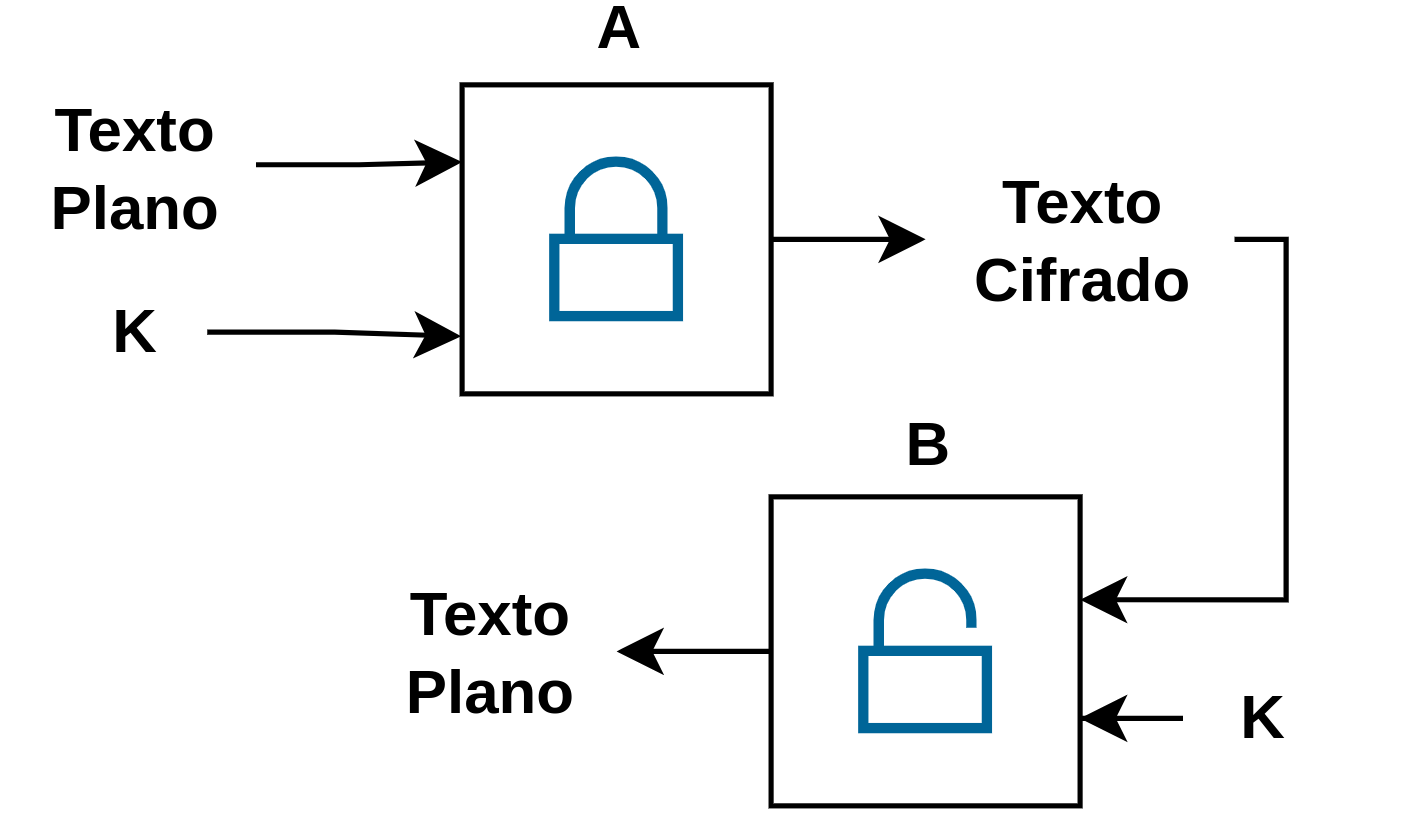
\includegraphics[width=\textwidth]{../figs/1_sim_encr.png}
        \caption{Encriptación simétrica}
        \label{fig:simetrica}
    \end{subfigure}
    \hfill
    \begin{subfigure}[b]{0.45\textwidth}
        \centering
        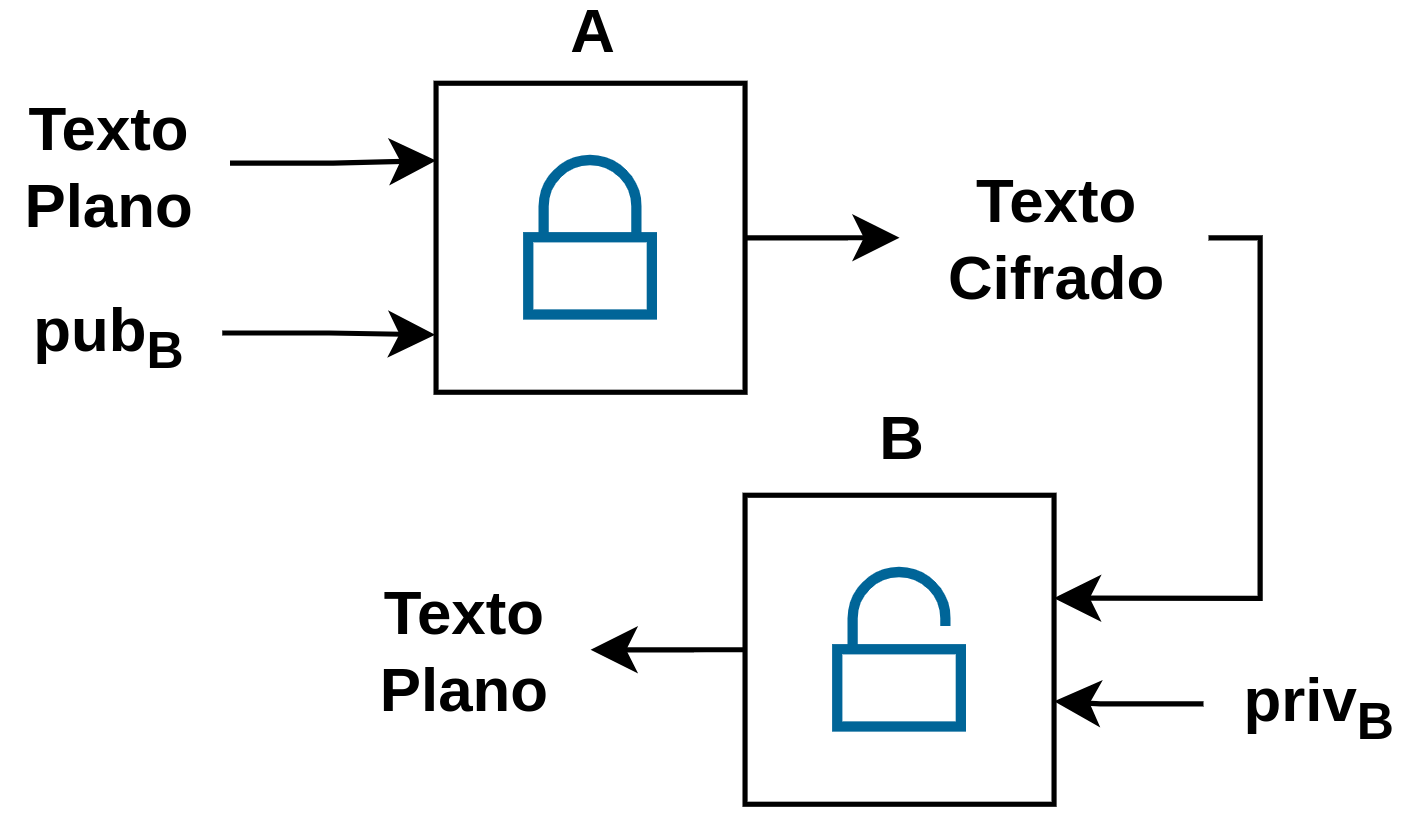
\includegraphics[width=\textwidth]{../figs/1_asim_encr.png}
        \caption{Encriptación asimétrica}
        \label{fig:asimetrica}
    \end{subfigure}
    \caption{Comparación entre encriptación simétrica y asimétrica.}
    \label{fig:encriptacion}
\end{figure}

%DIFFIE-HELLMAN
%CITAR PAPER ORIGINAL (REF EN WIKIPEDIA)
% REVISAR
El método de Diffie-Hellmann propone combinar ambos enfoques para lograr acordar, empleando el concepto de encriptación asimétrica, una clave simétrica de manera segura que puede ser usada posteriormente para encriptar información. La principal ventaja del método radica en que ambas partes logran generar la misma clave simétrica sin transmitirla por el canal, mitigando un gran problema de seguridad del enfoque simétrico. La figura \ref{fig:diffie-hellmann} describe las operaciones matemáticas sobre las cuales funciona el método de Diffie-Hellmann.

\begin{figure}[h!]
    \centering
    \includegraphics[width=0.4\textwidth]{example-image}
    \caption{Método de Diffie-Hellmann para el acuerdo de una clave común.}
    \label{fig:diffie-hellmann}
\end{figure}

% MODIFICAR ESTO (LA CIA MODERNA UTILIZA COMBINACIONES DE DIFERENTES ALGORITMOS)
Para los estándares de seguridad actuales, un esquema de establecimiento de comunicaciones requiere mayor complejidad para abordar desafíos como un ataque de tipo man-in-the-middle. Aún así, el método de Diffie-Hellmann es la base de numerosas implementaciones por su simplicidad y el elevado costo computacional que supone calcular la clave K conociendo únicamente las claves públicas A y B.

\subsection{Suposiciones y restricciones}
Distintas soluciones de encriptación pueden proponerse según la capa del modelo OSI que se analice. La encriptación a nivel de capa física minimiza las penalidades en rendimiento a costa de introducir complejidad al sistema, que se manifiesta en la necesidad de hardware dedicado de extremo a extremo de la red. Esta restricción puede volver inviable la encriptación a nivel de la capa física cuando el sistema de comunicaciones requiere de escalabilidad, principalmente por el costo de despliegue y mantenimiento.
La encriptación en capas superiores provee mayor flexibilidad en la implementación del sistema. Si bien esto introduce una mayor latencia a la red, reduciendo el rendimiento de la misma, se pueden lograr valores aceptables de latencia con suficiente optimización.  
Las soluciones de encriptación en la capa 3 tienen la ventaja de ser independientes de la capa física, reduciendo la complejidad del sistema y permitiendo mayor flexibilidad en la implementación y compatibilidad con infraestructura preexistente. Esto implica que, cualquier sitio que cuente con una conexión a Internet y un dispositivo de encriptación tiene la infraestructura suficiente para acceder a una red segura, denominada red privada virtual.

En sistemas de criptografía, usualmente se utiliza el concepto de dominios rojo/negro para describir las partes del sistema que trabajan con información legible (dominio rojo) y aquellas que contienen información cifrada (dominio negro). La arquitectura de un sistema de comunicación seguro debe tener en cuenta este concepto para una correcta segregación de dominios, mitigando así la posibilidad de filtraciones indeseadas de información. La normativa actual que refiere a la segregación de dominios no contempla la segregación virtual, es decir, contener en un mismo dispositivo ambos dominios y aislarlos empleando herramientas de software. El implementar un sistema de este estilo capaz de cumplir las normas de seguridad existentes es un desafío importante.



\subsection{Resumen del sistema propuesto}

El sistema de comunicaciones seguras que se propone contempla el diseño de un único dispositivo, denominado encriptador, con la capacidad de formar un túnel VPN entre redes preexistentes, asegurando ciertos estándares de autenticación y confidencialidad sobre las comunicaciones entre dichas redes. El sistema opera a nivel de capa 3 del modelo OSI, y requiere de un mínimo de dos encriptadores para su funcionamiento, aunque también se encuentra prevista la escalabilidad del sistema.
El propósito del sistema es brindar confiabilidad respecto a la autenticación, confidencialidad e integridad de la información transmitida entre redes interconectadas,  afectando al mínimo el rendimiento de la red.

\begin{figure}[h!]
    \centering    
    \includegraphics[width=0.4\textwidth]{example-image}
    \caption{Esquema simplificado del sistema de comunicaciones seguras.}
    \label{fig:overview}
\end{figure}

En el esquema de la figura \ref{fig:overview} se describen los denominados dominios rojos, correspondientes a redes donde se trata con información sensible. El complemento de estos se denominan dominios negros, que usualmente se consideran canales inseguros donde la información proveniente de un dominio rojo requiere estar encriptada. 
El dispositivo encriptador actúa de interfaz entre dominios rojo y negro, motivo por el cual gran parte de la seguridad del sistema recae sobre este. Este dispositivo cuenta con acceso a claves utilizadas para establecer sesiones seguras con otros dispositivos, y al mismo tiempo cuenta con acceso a Internet. Debe poder garantizarse la seguridad en la gestión de estas claves y rechazar accesos no autorizados al dominio rojo.

\clearpage

\subsection{Objetivos, metas y justificación del sistema}

Un dispositivo en el cual los dominios rojo y negro no estén correctamente segmentados se encuentra con que la información confidencial respecto al túnel VPN como claves y permisos se hallan expuestos en el caso de una intrusión desde Internet o desde la propia red interna. Esto lleva a la posibilidad de que un agente no autorizado sea capaz de desencriptar y modificar información que viaje por el túnel, así como también acceder a dispositivos dentro de una organización.

En el diseño del encriptador, se propone implementar la segmentación virtual de dominios rojo/negro, esto es, representar los dominios como entidades virtuales independientes que ejecutan sobre hardware compartido. Este concepto puede implementarse a través de los denominados hipervisores, software que permite que varios sistemas operativos independientes trabajen juntos, compartiendo los mismos recursos físicos.

La segmentación permite que la entidad negra, la cual está conectada a Internet, realice el control del tráfico y oculte la existencia de la entidad roja para cualquier servicio fuera de la red virtual privada. Por otro lado, la entidad roja es la responsable de encriptar/desencriptar las comunicaciones entre organizaciones que se encuentren dentro de la red privada y de gestionar las claves de encriptación y los privilegios de usuarios. Esta segmentación permite un control estricto sobre el tráfico entre ambas entidades, mitigando la posibilidad de transferir información como claves contenidas en la entidad roja hacia la entidad negra.


\subsection{Usuarios y modos de operación}

\begin{center}
    \textbf{Usuarios}
\end{center}

\begin{itemize}
    \item \textbf{Administrador de red}: responsable de la configuración y mantenimiento del encriptador. Cuenta con acceso a la interfaz de administración del dispositivo y es el encargado de configurar el encriptador para funcionar dentro de la red segura. La configuración del encriptador incluye la definición de las redes que se conectarán a través del túnel VPN, la configuración de las claves de encriptación y la definición de los permisos de los usuarios.
    \item \textbf{Usuario final}: utiliza la red segura para compartir información sensible a otros nodos de la red. No tiene acceso a la configuración del encriptador y su interacción con el sistema se limita a utilizar la red segura como si de su red local se tratase.
\end{itemize}

\begin{center}
    \textbf{Modos de operación}
\end{center}

El diseño prevee que, una vez configurado el dispositivo, la operación del encriptador sea transparente para el usuario final, el cual no necesita interactuar con el dispositivo para utilizar la red segura.
\begin{itemize}
    \item \textbf{Nodo pequeño:} este modo de operación es de utilidad en sitios que no cuentan con infraestructura de red. El encriptador opera también como router, procesando todo el tráfico del sitio y permitiendo que el tráfico no destinado a otro sitio de la red segura sea enrutado por fuera del túnel VPN. Esta funcionalidad es conocida como \textit{split tunneling}. Es adecuado para instalaciones con tráfico moderado.
    \item \textbf{Nodo grande:} en instalaciones con tráfico elevado y que posiblemente cuenten con una infraestructura de red acorde, el equipo únicamente opera como encriptador de las comunicaciones seguras, y se conecta a un router preexistente para las comunicaciones no seguras. De esta manera solamente el tráfico dentro de la red segura es procesado por el encriptador.
\end{itemize}

\begin{figure}[h!]
    \begin{subfigure}{0.45\textwidth}
        \centering
        \includegraphics[width=\textwidth]{example-image-a}
        \caption{Sitio sin infraestructura de red.}
        \label{fig:small_node}
    \end{subfigure}
    \hfill
    \begin{subfigure}{0.45\textwidth}
        \centering
        \includegraphics[width=\textwidth]{example-image-b}
        \caption{Sitio con infraestructura de red.}
        \label{fig:large_node}
    \end{subfigure}
    \caption{Modos de operación del encriptador.}
    \label{fig:modes_of_operation}
\end{figure}

\section{Requerimientos}
El documento de requerimientos es utilizado para describir que necesita el sistema para cumplir las necesidades de los usuarios. Esta sección establece las bases para la solución propuesta. Se definen a continuación las palabras clave que se utilizarán para referirse a los requerimientos:

\begin{table}[h!]
    \centering
    \begin{tabular}{|l|p{10cm}|}
        \hline
        \multicolumn{1}{|c|}{\textbf{Palabra clave}} & \multicolumn{1}{c|}{\textbf{Descripción}} \\
        \hline
        \textbf{DEBE} & Indica un requerimiento obligatorio que debe cumplirse para que el sistema funcione correctamente. \\
        \hline
        \textbf{NO DEBE} & Indica un requerimiento que no debe cumplirse, es decir, una restricción que debe evitarse. \\
        \hline
        \textbf{DEBERÍA} & Indica un requerimiento recomendado, pero no obligatorio. Se sugiere cumplirlo para mejorar la calidad del sistema. \\
        \hline
        \textbf{NO DEBERÍA} & Indica un requerimiento que se desaconseja cumplir, pero no es obligatorio evitarlo. \\
        \hline
        \textbf{PUEDE} & Indica una opción o característica que el sistema puede implementar, pero no es obligatoria. \\
        \hline
    \end{tabular}
    \caption{Palabras clave utilizadas en la definición de requerimientos.}
    \label{tab:palabras_clave_requerimientos}
\end{table}
\subsection{Funcionales}

\begin{itemize}
    \item \textbf{Renovación de claves:} cada par de nodos realiza una renovación de claves efímeras cada 120 segundos para asegurar forward-secrecy. Esto significa que, si una clave es comprometida por alguna razón, no se comprometen las comunicaciones anteriores o futuras fuera del intervalo de tiempo especificado.
    \item \textbf{Seguridad ante intrusiones:} el equipo debe ser capaz de  mitigar la posibilidad de intrusiones de agentes no autorizados vía software, tanto desde Internet o como desde la red local.
    \item \textbf{Detección de ataques DoS:} el sistema debe ser capaz de detectar y mitigar ataques de denegación de servicio.
    \item \textbf{Movilidad:} el sistema debe ser capaz de soportar la movilidad de los nodos y permitir a un nodo moverse entre redes sin interrupciones ni renegociaciones de claves. 
    \item \textbf{Split-tunneling:} el sistema debe ser capaz de permitir y enrutar tráfico de ciertas aplicaciones o servicios por fuera del túnel VPN. 
    \item \textbf{Segmentación de dominios: } el sistema debe aislar procesos contenidos en un dominio de información, como pueden ser archivos, contenida en otro dominio, independientemente de los privilegios que tenga este proceso.
\end{itemize}

\subsection{De rendimiento}

\begin{itemize}
    \item \textbf{Tasa de transferencia:} el sistema debe ser capaz de lograr, de un nodo a otro, una tasa de transferencia de 950 Mbits/s de datos planos.
    \item \textbf{Número de nodos:} una red segura debe ser capaz de soportar hasta 250 dispositivos encriptadores, también denominados nodos. 
\end{itemize}

\subsection{De interfaz}

\begin{itemize}
    \item \textbf{Administración:} la configuración de funcionamiento del  encriptador debe poder ser modificada únicamente por un administrador de red autorizado de manera local.
    \item \textbf{Interfaz de usuario:} el sistema debe ser transparente para el usuario final, es decir, no debe requerir de configuraciones adicionales para este.
    \item \textbf{Configuración de operación:} el modo de operación en red del sistema y otros parámetros de funcionamiento asociados deben ser configurables únicamente por el administrador de red.
\end{itemize}
\clearpage

\section{Descripción de tecnologías}
En este trabajo se combinarán distintas tecnologías que conformarán la solución final. A continuación se describen brevemente a modo de contextualizar al lector.

\subsection{WireGuard}
WireGuard es un protocolo de túneles VPN derivado de Noise Protocol Framework. Está diseñado para ser simple, rápido y eficiente, proporcionando una solución de código abierto con una base de código pequeña, lo que ayuda a minimizar la superficie de ataque. Su propósito es proporcionar una alternativa segura y eficiente a los protocolos VPN tradicionales, permitiendo la creación de túneles seguros entre dispositivos en una red. 

% Ejemplo de un archivo de configuración wg0.conf
\subsection{seL4}
Se trata de un microkernel con verificación formal matemática que garantiza que su implementación está libre de errores. Cuenta con una base de código muy reducida y proporciona un fuerte aislamiento entre procesos y una interfaz de comunicación segura. Es utilizado en sistemas críticos donde la seguridad y la confiabilidad son fundamentales. 

\subsection{CAmkES}
Trabajar con un microkernel como seL4 implica que la mayoría de las funcionalidades del sistema deben implementarse en el espacio de usuario. Para simplificar este proceso, seL4 incluye CAmkES, un \textit{framework} que facilita el desarrollo de sistemas de software modulares y seguros, diseñados específicamente para ejecutarse sobre seL4.

% \textcolor{blue}{Modular refiere a que CAmkES es un modelo de componentes. Seguro refiere a. Detallar el componente VMM, será utilizado después.}

% \begin{figure}[h!]
%     \centering
%     \includegraphics[width=0.5\textwidth]{example-image}
%     \caption{VMM.}
%     \label{diag:camkes_vmm}
% \end{figure}

% VirtQueue

% Comunicación VM - VMM - seL4 - Hardware

\noindent\rule{\textwidth}{0.4pt}

\subsubsection{zmq\_samples}
Uno de los ejemplos de uso de VMs en CAmkES es el proyecto zmq\_samples, que implementa un sistema de comunicación entre VMs utilizando la librería de mensajería ZeroMQ. Cada VM contiene una interfaz de red virtual eth0 que se conecta a las interfaces eth0 de las demás. En la figura \ref{diag:zmq_samples} se esquematiza el funcionamiento de este sistema.
\pdfcomment{esto va en otro lado}

\begin{figure}[h!]
    \centering
    \includegraphics[width=0.5\textwidth]{example-image}
    \caption{Esquema de comunicación zmq\_samples.}
    \label{diag:zmq_samples}
\end{figure}

